\documentclass[11pt]{article}
\usepackage[french]{babel}
\usepackage[T1]{fontenc}
\usepackage{fontspec}
\usepackage[utf8]{inputenc}
\usepackage{url}
\usepackage{eurosym}
\usepackage{pdfpages}
\usepackage{ulem} % to use a strikeout/strikethrough font
\usepackage{color}
\newcommand{\fs}[1]{\textcolor{red}{\sout{#1}}}
\newcommand{\f}[1]{\textcolor{blue}{#1}}
\usepackage{graphicx} % Inclure des images
\usepackage{multicol} % Multi-colonnes


\usepackage[autolanguage, np]{numprint} % écriture des virgules
\usepackage[top=3cm,right=2cm,bottom=2cm,left=2cm]{geometry}

\title{HAUM}
\author{Assemblées Générales Ordinaire \& Extraordinaire}
\date{6 Février 2018}

\begin{document}
\maketitle

\section*{Convocation}

Madame, Monsieur,

L'association HAUM vous convoque à ses Assemblées Générales Ordinaire \& Extraordinaire qui se tiendront le :

\begin{center}
{\Large 6 Février 2018 à 19h00}\\
à Le Mans Innovation,\\57 Bd Demorieux au 2\textsuperscript{ème} étage,\\72 100 Le Mans
\end{center}

En cas d'impossibilité, veillez vous faire excuser et vous faire représenter si vous le souhaitez (2 procurations maximum par personne présente, Statuts, art. 6).

\vspace{1.5cm}

\hrule
\vspace{.3cm}
\begin{center}
\Large\bfseries Assemblée Générale Extraordinaire
\end{center}
\vspace{.3cm}
\hrule

\vspace{1.5cm}

\section*{Déroulement}

\begin{enumerate}
    \item Appel et annonce des procurations
		\item Questions diverses
\end{enumerate}

\section*{Clotûre}

\vspace{1.5cm}

\hrule
\vspace{.6cm}
\begin{center}
\Large\bfseries Assemblée Générale Ordinaire
\end{center}
\vspace{.3cm}
\hrule

\vspace{1.5cm}

\section*{Déroulement}

\begin{enumerate}
    \item Présentation de l'association
    \item Rapport moral
        \begin{enumerate}
            \item Bilan
            \item Objectifs
            \item Questions
        \end{enumerate}
    \item Rapport financier
        \begin{enumerate}
						\item En images
            \item Bilan \& Objectifs
            \item Questions
        \end{enumerate}
    \item Motions et vote
    \item Élection du nouveau bureau
    \item Questions diverses
\end{enumerate}

Vous trouverez en annexe au présent document le budget prévisionnel 2018.

\section{Présentation de l'association}

\section{Rapport Moral}

\subsection{Bilan}

\subsubsection{Le Mans Innovation \& déménagement}
Une fois de plus, l'année passée a été riche en changements, projets et évènements. Au
premier plan, il faudra retenir de 2017 qu'elle fut une année de déménagement. Le HAUM
quitte ainsi le 19 Boulevard Oyon pour prendre ses quartiers au 57 Boulevard Demorieux, au
sein de Le Mans Innovation (LMI).
Le nouveau local comprend deux salles pour un total d'environ 120m\textsuperscript{2}. La
plus grande des deux accueil un espace "propre" comprenant entre autres la paillasse
électrique, le Free to Hack et une vitrine permettant de présenter les activités. Le
second (atelier "sale") accueille le stock de matières premières, la fraiseuse, les scies
\& perceuses.

Dans le cadre de LMI, l'espace fablab (occupé par le HAUM) a été équipé
d'une découpeuse LASER (Robotseed, 600$\times$400mm de surface utile) et d'une imprimante 3D
(Ultimaker 2+ Extended). Ces équipements sont à disposition du HAUM et leur maintenance
sous sa responsabilité.

Des partenariats avec des résidents de LMI ont vu le jour, le local est ainsi utilisé en
journée par Bertrand (Chaines de Pluie, atelier propre) et Marc (Furion Motorcycles,
atelier salle). Divers ajustements quant au partage des tâches sont à prévoir dans
l'avenir pour que le local reste propre et soit utilisé au mieux, toutefois, ces
rapprochements sont prometteurs.

Reste à définir également les modalités de contrôle de l'accès au local. La présence de
matériel dangereux pose la question de comment limiter le risque de blessures et préserver
les machines. Lors de plusieurs discussions en séance, il a été convenu de mettre en place
un contrôle d'accès au local par badge. Il s'agit d'un projet en cours de réalisation
prévu pour une installation au plus tôt. Dans le cadre de la protection du matériel il a
également été évoqué de changer les canons : des doutes planent sur d'éventuels doubles
des clés ayant pu être réalisés sans le consentement du HAUM ou de LMI.

Dans cette fin d'exercice, le bureau du HAUM s'est attaché à réguler l'accès de personnes
non membres aux machines et au lieu suite à de sérieux doutes sur les activités de
certains (d'un point de vue légal entre autres).

\subsubsection{Evènements}

Le HAUM a cette année encore participé à de nombreux évènements et proposé autant de
projets innovants. Voici les plus marquants.

\paragraph{HAMExpo} Sur une invitation de l'Électrolab (Nanterre), le HAUM a participé à
HAMExpo, salon de radioamateurs organisé au Mans en 2018. Les membres présents ont pu
échanger avec la communauté des RA et avec quelques membres de l'Électrolab.

\paragraph{Teriaki} Le festival Teriaki s'est, comme à l'accoutumée, déroulé à la fin
août. Le HAUM était présent avec un nouveau labyrinthe appelé "Féroce". Sur le même
principe que le labyrinthe Initiati proposé en 2016, il s'agit d'un dédale multi-états,
matérialisé au sol. Contrairement à l'an dernier, l'animation, placée en plein soleil et
loin des lieux principaux du festival, a été moins fréquentée.

Le HAUM présentait également un remix du dHAUM/dHAUMidi ... appelé dHAUMadi (désolé). Le
projet avait été prévu pour n'être pas d'un niveau technique trop élevé afin de permettre
à de nouveaux membres de s'impliquer dans la vie de l'association.  Malgré ce point, le
projet n'avançant pas, les mêmes membres que d'habitude se sont attelés à la tâche et ont
réussi à produire un jeu à taille humaine très apprécié du public. Merci à eux !

\paragraph{Festival D} L'édition 2017 du festival était organisé par Ping et l'ESBA-TALM
au Quai d'Angers. Elle a rassemblé de nombreuses structures présentant des projets
innovants allant de la tricoteuse numérique à l'open-data musicale en passant par divers
robots et machines. Le HAUM y a présenté à nouveau dHAUMadi qui avait été développé pour
Teriaki peu avant.

Les discussions au cours du festival ont été intéressantes. En particulier, des
discussions avec MyHumanKit (Rennes) ont été engagées autour du développement d'un capteur
myoélectrique libre. Quelques développements et recherches en ce sens ont commencé,
beaucoup reste à faire.

\paragraph{24h du code} Le HAUM a réitéré sa participation aux 24h du code en proposant
une nouvelle arène. Le sujet, répondant au nom de Marabunta\footnote{Traduit parfois
"fourmi légionnaire"}, portait sur l'écriture d'une intelligence artificielle
multi-agents. Un programme devait contrôler tour à tour une fourmilière et les différentes
fourmis disposant chacune de capacité et d'une mémoire minimales. Les équipes jouant le
sujet ont plutôt bien réussi et apprécié le défi. Le maintien de la participation du HAUM
est grandement liée à l'implication de Florent ainsi que Laurent \& Corentin. Merci
grandement à eux.

\paragraph{Jeudi du Libre} L'année 2016 a montré la limite des jeudi du libre : beaucoup
de discussions certes mais peu en rapport avec le logiciel libre ou le hack. Il avait été
montré à l'AG 2016 que le format ne convenait plus aux attentes d'une bonne partie des
membres actifs. Il fut alors proposé de changer le format et d'inciter chacun à venir
présenter aux jeudis du libre un logiciel ou une pratique qu'iel connaît/affectionne
autour d'une bière. Ce format a commencé correctement avec une présentation de Wikimedia
entre autres mais a rapidement périclité faute de présentateurs motivés avant de mourir
avec la cession de l'Épicerie à l'été.

\subsubsection{Projets et axes}

Il y a plusieurs projets en cours. Au niveau collectif (pour des projets qui occupent
quelques personnes) on a aujourd'hui:

\begin{description}
	\item[Photographie] Sténopé, stéréo-photographie, etc\ldots
	\item[Lumière] Plusieurs projets également : scratch holograms, light painting,  moirés, Tål
	\item[IdiHAUM] Solution de contrôle d'accès
\end{description}

Les réunions "projets" qui avaient été proposées et instaurées lors de la dernière années
ont été plutôt bien suivies et utiles au début de l'exercice et ont complètement disparu
pendant l'été. Elle permettaient à tous de s'informer des projets en cours régulièrement
et une solution de remplacement est peut être à chercher.

\subsection{Objectifs}

Au cours de l'année 2018, le bureau du HAUM chercher à réorienter l'association vers des
projets plus techniques, souhaitant ainsi contenter ses plus anciens membres. Alors que la
politique des dernières années était axée vers l'attrait de nouveaux membres et la
croissance de l'association, de nombreux membres (très actifs sur les projets) s'en
sentent frustrés.

Pour plus de contexte, il est arrivé plusieurs fois au cours des dernières année que les
projets soient bridés d'un point de vue technique afin de faciliter la participation de
memebres moins expérimentés. Cette auto-censure du HAUM sur les solutions envisagés pose
le problème du contentement des membres les plus actifs de l'association (techniquement
plus avancés). Si chacun vient au HAUM pour apprendre et se développer, il semble
essentiel de viser toujours plus haut et de compter sur l'entraide pour emmener les moins
expérimentés. Une remarque qui revient régulièrement est que, dans tous les projets, il y
a des parties moins techniques et donc plus abordables.

Au cours de l'année, la question des projets à échéance s'est posée. En effet, le HAUM
s'engage dans de nombreux projets avec de nombreux partenaires. Ces projets sont toujours
largement acclamés et encouragés mais mettent une pression importante sur le petit nombre
de membres actifs. Une décision s'est prise \textit{de facto} au cours des séances, les
projets avec une deadline seront à éviter à l'avenir.

Une discussion qui est revenue récemment au HAUM porte sur l'organisation d'un Hacker Camp
sans public pour rencontrer et rigoler avec les bidouilleurs venus d'ailleurs. Ce camp a
été proposé indépendamment par des membres de l'Électrolab, un visiteur régulier du HAUM
et des membres du hackerspace. Quelques tracts ont pu être distribués au cours du FOSDEM
pour sonder les envies d'autres. Tout reste à faire mais c'est plutôt prometteur\ldots

Lors de Festival D, les responsables du festival ont plusieurs fois évoqué le fait de
faire la prochaine édition au Mans. Ce point n'a pas été grandement discuté au sein du
hacklab mais il s'inscrirait bien dans la dynamique, permettant de faire de la diffusion
et de la médiation vers le grand public un sujet actif sans diminuer la technicité des
projets. Cette possibilité est à évaluer, mais il faut savoir que l'organisation du
festival demande aujourd'hui à Ping de recruter une personne à plein temps pendant un an
(en service civique).

Devant les difficultés que peuvent avoir les nouveaux membres à s'intégrer et les anciens
à suivre l'évolution des projets, le bureau à cherché une solution. Les discussions ont
mené à proposer un "HackPairHAUM", sorte d'apéro bimensuel où les membres peuvent venir
échanger hors du local et auquel les nouveaux sont invités à venir découvrir
l'association. Ce genre d'évènement pourrait, d'après le bureau, avoir l'avantage de
casser la barrière entre nouveaux et anciens sans frustrer ceux qui veulent continuer à
avancer sur leur projet. Il répond aussi à la disparition du côté social des jeudi du
libre et des réunions "projets" en proposant un évènement unique de remplacement.
Finalement, aux yeux du bureau, des temps conviviaux manquent et sans eux, impossible de
cristalliser une communauté. Des regroupements de ce genre nous semblent essentiels.

\section{Rapport financier}

\subsection{En images}
Nous présentons ici le bilan financier de l'année 2017.
\begin{center}
%\begin{multicols}{2}
%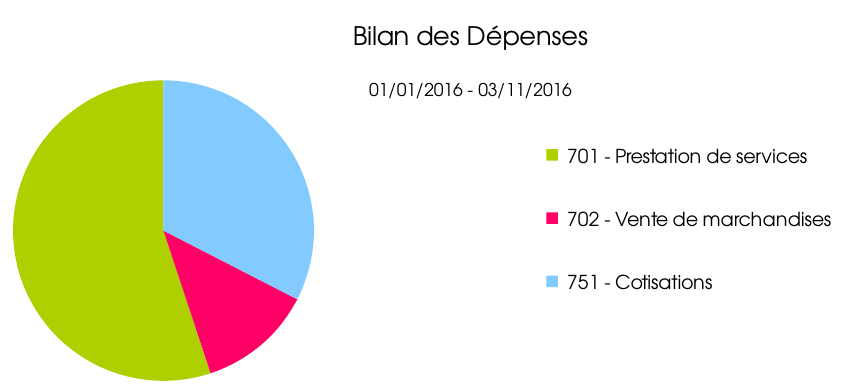
\includegraphics[width=8cm]{1DossierAGRecettes.png}

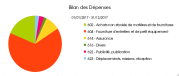
\includegraphics[width=8cm]{2DossierAGDepenses2017.png}
%\end{multicols}

\begin{multicols}{2}
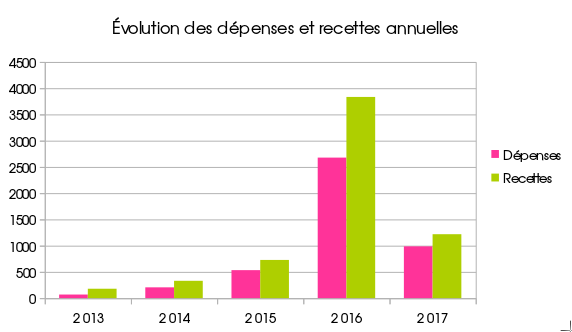
\includegraphics[width=8cm]{3DossierAGGeneral2017.png}

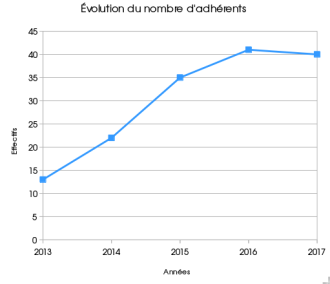
\includegraphics[width=8cm]{4DossierAGAdherents2017.png}
\end{multicols}
\end{center}
\subsection{Bilan et objectifs}
Après une année 2016 en forte croissance, il y a eu une stabilisation des volumes
financiers en 2017.

Dans la continuité de l'an passé, nous avons poursuivi l'objectif de mutualisation
des moyens matériel. Le Mans Innovation nous a mis à disposition une découpeuse laser
dans notre local et nous avons investi dans une machine à tricoter, un routeur
et une Kress.

Si on souhaite être en capacité de financer des machines ou de l'outillage plus onéreux
ou en plus grand nombre, l'augmentation des cotisations, des mécénats et/ou des
actions qui seraient capables de nous rapportés de l'argent seraient les bienvenus.

Cette année, les dépenses ont été effectuées en suivant rigoureusement les règles
instaurées depuis 2 ans maintenant. La gestion de trésorerie fut donc plus aisée.

Pour continuer dans cette dynamique, nous rappelons ici les règles de fonctionnement :
\begin{itemize}
 \item toutes les factures doivent être établies \textbf{au nom du HAUM} et ne
 contenir que des éléments \textbf{achetés pour le HAUM} ;
 \item les dépenses de l'argent du hackerspace ne doivent être faites qu'après
 \textbf{consultation des autres membres} et, surtout, \textbf{vérification de la
 trésorerie} ;
 \item une demande de validation \textbf{par mail} doit être effectuée.
\end{itemize}

Le bilan financier contient, à ce jour, deux impayés : un premier de 250\euro{}
(concernant un chèque refusé à trois reprises) et un second de 300\euro{} (Prestation
Teriaki).

\paragraph{Prévisions 2018}
Pour l'année à venir, le budget prévisionnel a été construit sur la base des charges
et des recettes de l'année 2017.

\subparagraph{Recettes}
Il est estimé pour les recettes :
\begin{itemize}
 \item 300\officialeuro~ de prestations ;
 \item 1200\officialeuro~ de cotisations.
\end{itemize}

\subparagraph{Charges}
Pour les charges, il est prévu :
\begin{itemize}
 \item 265\officialeuro~ pour l'achat de fournitures ;
 \item 700\officialeuro~ pour les petits équipements ;
 \item 246\officialeuro~ pour les autres fournitures (par exemple, en 2016, les tee-shirts) ;
 \item 50\officialeuro~ pour la communication (cartes de visites, ...) ;
 \item 150\officialeuro~ pour les frais de déplacement, de réception, ...
\end{itemize}

\subparagraph{Bénévolat}La valorisation du bénévolat sera établie régulièrement lors des réunions mensuelles.
Elle a été estimée à \np{8142}\officialeuro~ pour l'année prochaine.

\subparagraph{}Le budget prévisionnel est alors de \np{18942}\officialeuro.

\section{Motions}
Aucun amendement au Règlement Intérieur n'a été proposé.

\section{Questions Diverses}

\newpage

\clearpage
\thispagestyle{empty}
\topskip0pt
\vspace*{\fill}
\begin{center}
\hrule
\vspace{.3cm}
\Huge\bfseries Annexes
\vspace{.3cm}
\hrule
\vspace{2cm}
\Large
\noindent Budget Prévisionnel 2018
\end{center}
\vspace*{\fill}

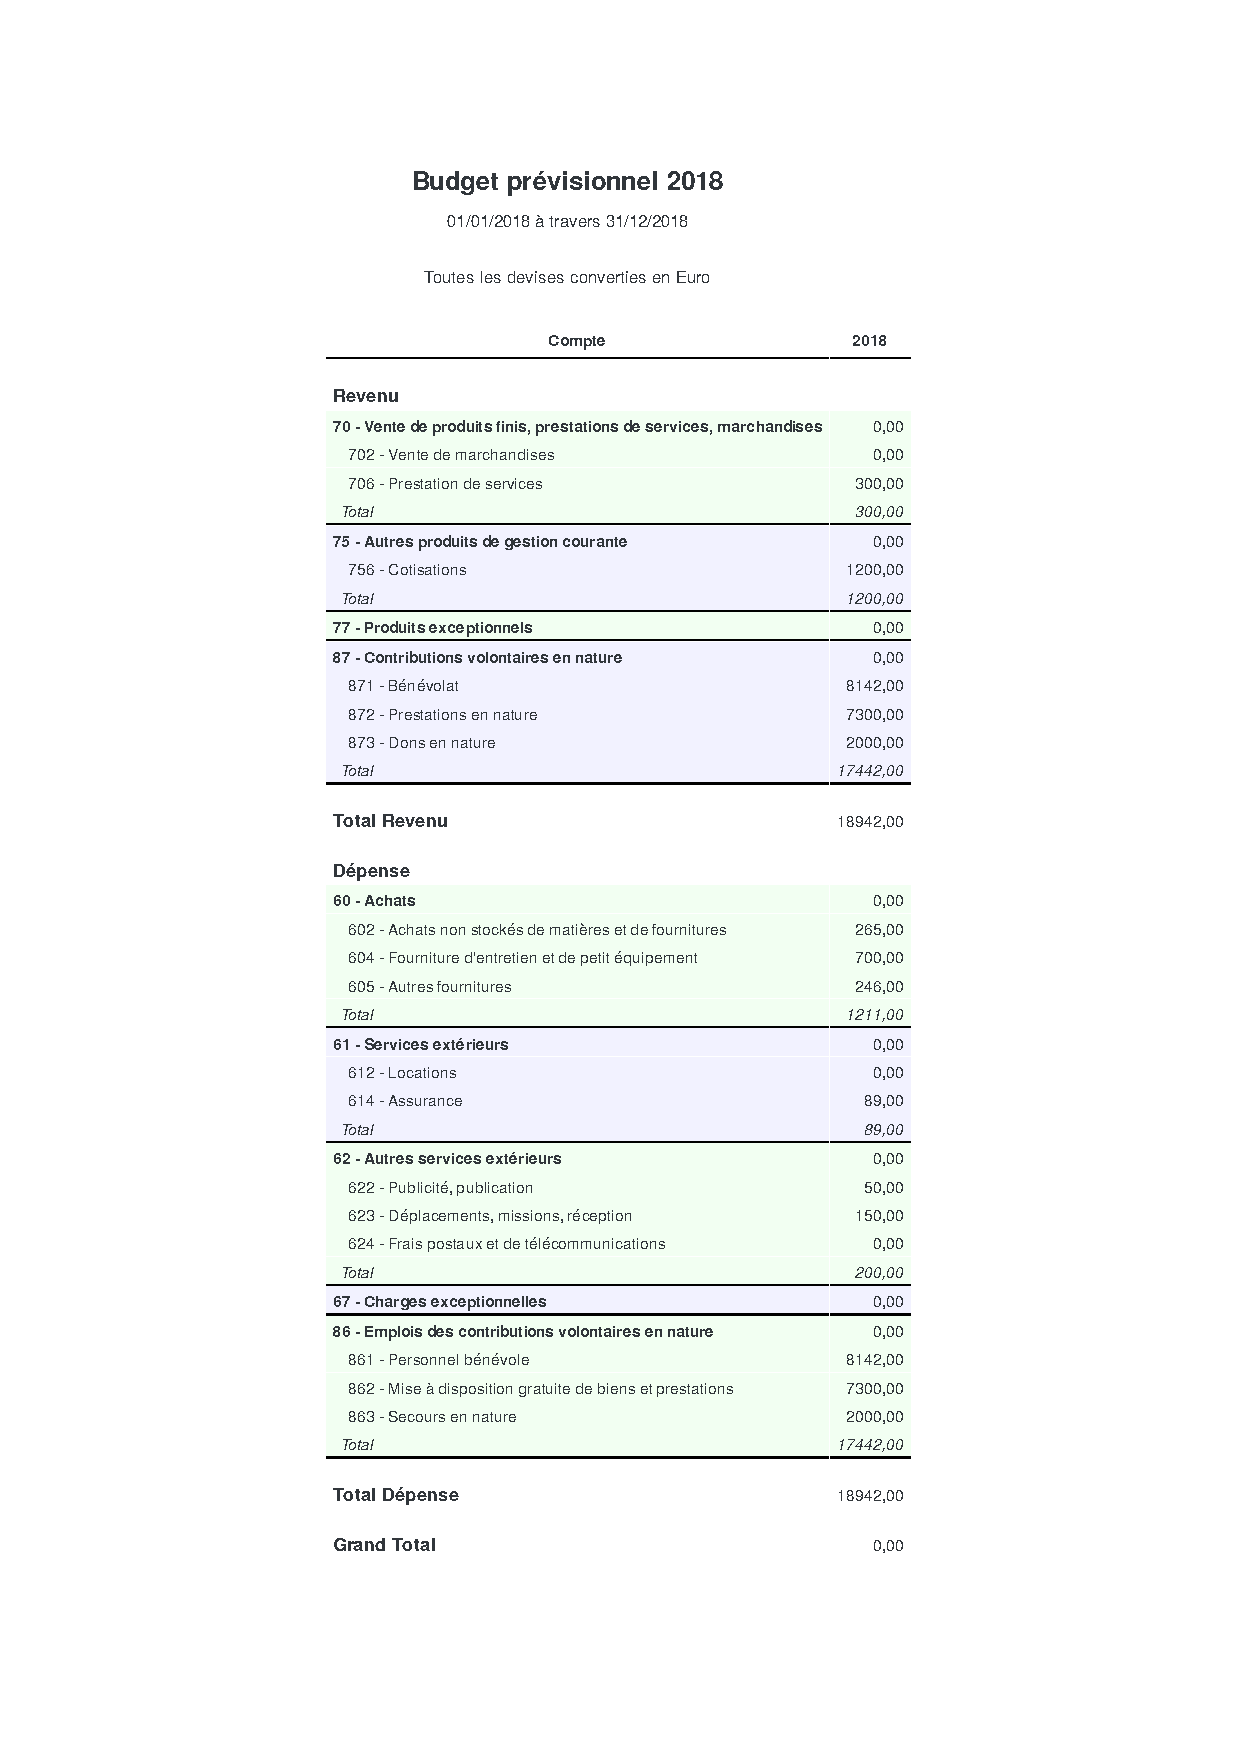
\includepdf[pages=-]{BudgetPrevisionnel2018.pdf}

\end{document}

% vim: set spelllang=fr:
